\section{Question 1}

The data are shown on \autoref{q1_two_observations}.

\begin{figure}[!ht]
  \centering
  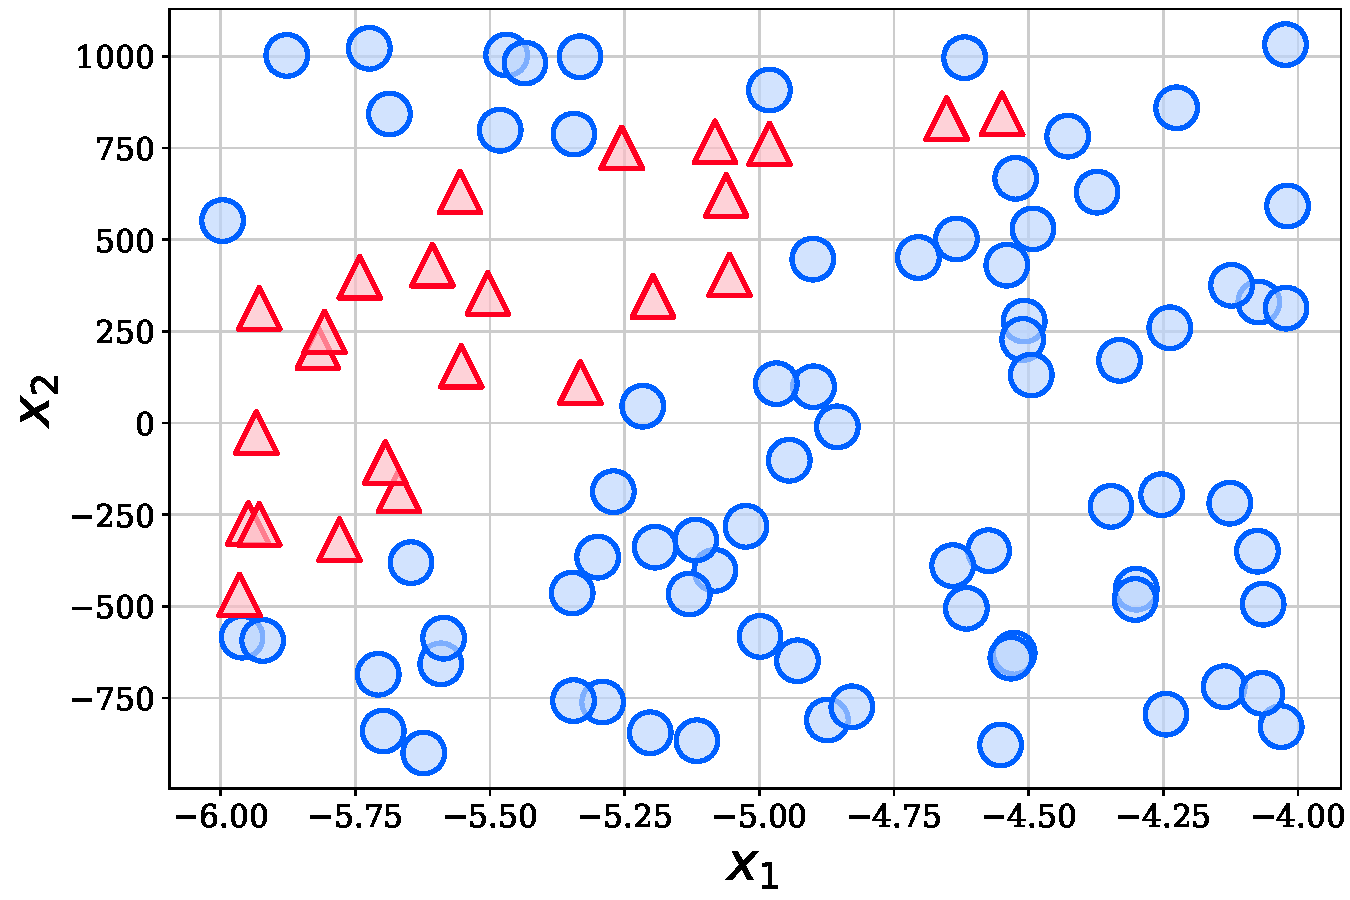
\includegraphics[width=0.8\textwidth]{figures/q1.pdf}
  \caption{Two types of observations. Code: q1.py.}
  \label{q1_two_observations}
\end{figure}

The diagram of the neural network is shown on \autoref{q1_network_diagram}. I choose the sigmoid activation function for the hidden layer nodes, because it's a common one. This is a classification task with just a single binary output (0 or 1). Therefore, for simplicity, I chose a single output node with no activation function (i.e. $f(x) = x$). If there were more than one output nodes than I could try a softmax function, but here it's not necessary.

\begin{figure}[!ht]
  \centering
  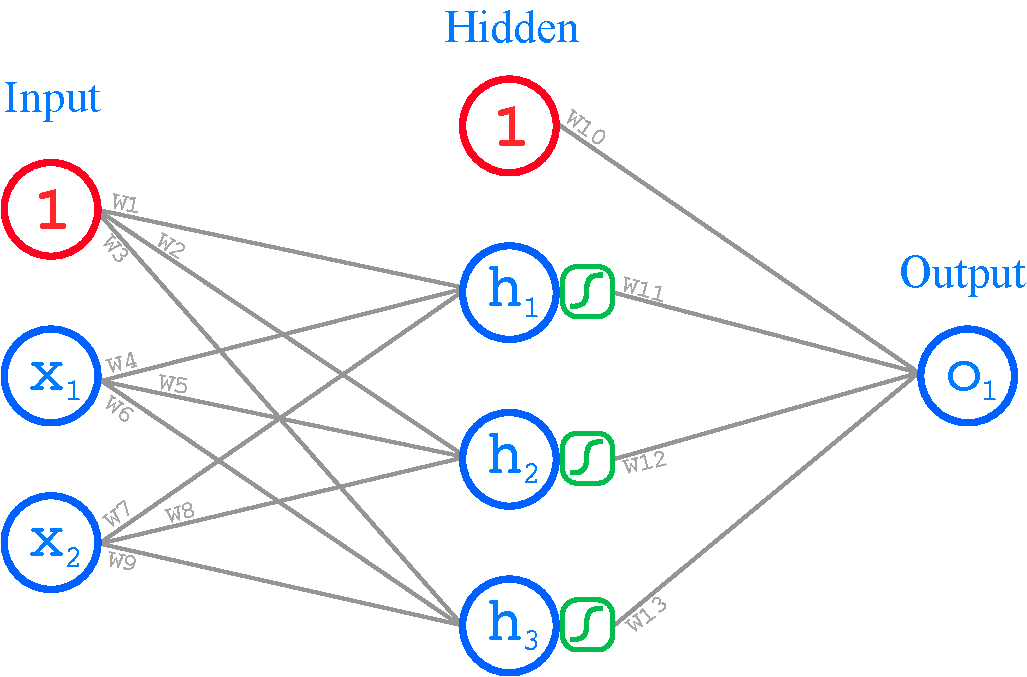
\includegraphics[width=0.7\textwidth]{figures/q1_neural_network.pdf}
  \caption{Diagram of the neural network containing two inputs, single hidden layer with three nodes and a single output layer.}
  \label{q1_network_diagram}
\end{figure}


\subsection*{Removing sigmoid from output layer}

In Lecture 13 example code (\url{http://astrowizici.st/teaching/phs5000/13/}), I removed the sigmoid for the output node (replacing it with $f(x) = x$). The reason I removed the sigmoid is the following. The output of the sigmoid is between 0 and 1, and this is used as predicted value from our model. However, in the loss function, we are comparing the predicted values with real values. The problem is that real value sometime outside the $[0, 1]$ range because they are normalized with mean $0$ and standard deviation of $1$. Consequently, the loss function will never approach zero. More importantly, the output of the model can not be used to generate the data.

I compare the loss function of the original and the modified models on \autoref{q1_lecture13_loss_compare}. We can see the modified model converges faster. The original will never converge to zero, even if we increase the number of interations.

\begin{figure}[!ht]
  \centering
  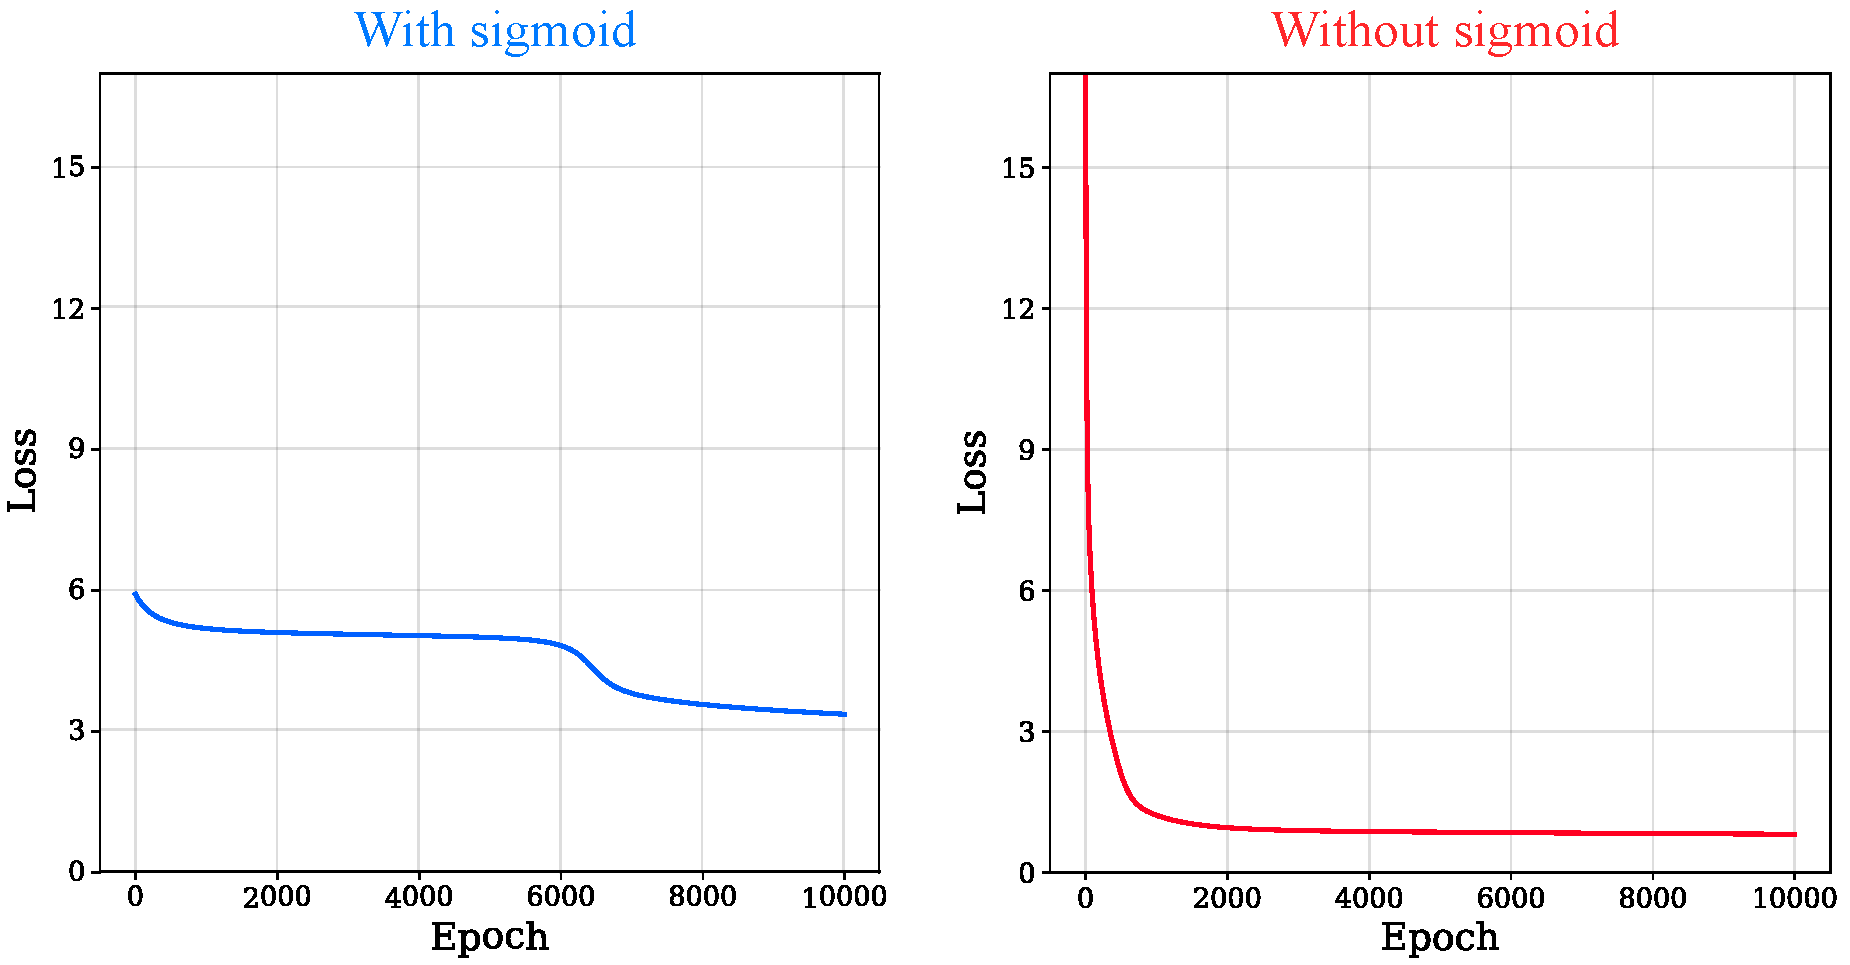
\includegraphics[width=1\textwidth]{figures/lecture13_loss_compared.pdf}
  \caption{Loss function for neural network from Lecture 13. The original code (left) contains sigmoid activation function in the output node, while the modified code (right) has no activation function ($f(x) = x$) in the output node. Both codes are otherwise identical, including the same seeding of random number generators.}
  \label{q1_lecture13_loss_compare}
\end{figure}

Original code: \\ \url{https://github.com/evgenyneu/ASP5020_data_analysis_problem_sets/blob/master/ps5/code/lecture13_original_with_signoid_output.py}

Modified code without output sigmoid: \\ \url{https://github.com/evgenyneu/ASP5020_data_analysis_problem_sets/blob/master/ps5/code/lecture13_remove_sigmoid_from_output.py}



